\chapter{Methodology}
\label{methodology}

This research considers seven trading methods to be compared: \textbf{buy-and-hold}, \textbf{MACD} indicator trading, two value-based model-free RL algorithms \textbf{DQN} and \textbf{Sarsa}, two policy-based model-free RL algorithms \textbf{A2C} and \textbf{A3C}, and one model-based RL algorithm \textbf{PETS}.

\section{Dataset}
All training and testing data \texttt{BTC} data in term of \texttt{USD}. A sole training dataset $\mathcal{D}_{train}$ is fetched from CryptoDataDownload \cite{DATA01}, containing 11,144 per-hour data points from to 14 October 2020 22:00 UTC to 22 January 2022 05:00 UTC. This date range is selected because it is a crab market with two bull markets and two bear markets.

Test datasets $\mathcal{D}_{test}$ are provided by Cryptocompare\footnote{https://www.cryptocompare.com/} API, consists of two sets of timeframes, namely:
\begin{itemize}
	\item Each-hour bull data (\texttt{HBu}): 2,000 points of data from 9 November 2022 06:00 UTC to 31 January 2023 14:00 UTC inclusive,
	\item Each-hour bear data (\texttt{HBr}): 2,000 points of data from 9 November 2021 06:00 UTC to 31 January 2022 14:00 UTC inclusive,
	\item Each-minute crab data (\texttt{MCr}): 2,000 points of data from 16 February 2023 04:40 UTC to 17 February 2023 14:00 UTC inclusive,		
	\item Each-minute bull data (\texttt{MBu}): 2,000 points of data from 14 February 2023 04:40 UTC to 15 February 2023 14:00 UTC inclusive.
\end{itemize}

Each data point contains five information:
\begin{itemize}
	\item \texttt{timeframe}: the time point where the price movement occured,
	\item \texttt{high}: the highest price recorded in that timeframe,
	\item \texttt{low}: the lowest price recorded in that timeframe,
	\item \texttt{open}: the price recorded at the start of that timeframe,
	\item \texttt{close}: the price recorded at the end of that timeframe.
\end{itemize}

The datasets go through a preprocessing step that adds three more custom columns to the original data, namely:
\begin{itemize}
	\item \texttt{ewm}: the value of $EMA(28)$ of that timeframe,
	\item \texttt{macd\_histo}: the values of $MACD(26,12,9) - SignalLine$ of that timeframe,
	\item \texttt{return}: the price movement since the last data point's close.
\end{itemize}

\section{Problem Representation}
Given a dataset $\mathcal{D}$ and an initial investment of \texttt{USD 10,000}. At each data point $d_t$ at timeframe $t$, a trading agent must decide to perform an action: either \texttt{BUY}, \texttt{SELL}, or \texttt{HOLD}. Since the setting is a spot trading environment, the agent is not allowed to buy more asset than its current unspent capital and is not allowed to sell more than the value of Bitcoin it holds. All trades are executed without transaction fees, following Binance's move\footnote{https://www.binance.com/en/support/announcement/binance-launches-zero-fee-bitcoin-trading-10435147c55d4a40b64fcbf43cb46329}. Finally, all agents are compared against another using the factors specified in Section \ref{sec:performancemx}.

\section{Performance Metrics}
\label{sec:performancemx}
Three performance metrics are used for final agent evaluation and also act as factors that determine reward\footnote{however, see \ref{rewardfn}}:
\begin{itemize}
	\item The average of portfolio return of agent $\alpha$ at all timeframes ($\phi_\alpha$) over benchmark return ($\phi_\odot$) = $average(\phi_\alpha - \phi_\odot)$, symbolized as $\overline{\Delta\phi_{\alpha,\odot}}$: larger is better,
	\item Maximum drawdown at the final timeframe $T$ (MDD$_T$): ranges from 0 to 1, closer to zero is better, and
	\item Non-annualized 100-timeframe Sortino ratio at the final timeframe $T$ ($\zeta_T$), larger is better.
\end{itemize}

To compare between agents, in addition to the above factors, one extra factor is included: 
\begin{itemize}
	\item Training speed ($s$), calculates the approximate time it takes for the training reward to converge in seconds, smaller is better. The number of episodes at the time point may follow.
\end{itemize}

\section{Non-RL Agents}
% how to perform the experiment
% Buy-and-Hold, MACD, RL algo in detail (implementation)
\subsection{Buy-and-Hold Agent}
The buy-and-hold agent is the bare basic agent as a global control variable, usually called as the ``benchmark" in algo trading. The strategy is simple: buy at the first timeframe and sell at the last timeframe. There is no learning or calculation involved. Directly using testing datasets, the portfolio return (as a ratio) of this agent is equal to $\frac{p_{2000} - p_0}{p_0}$, in other words, the price movement relative to the initial price. An agent can be called a profitable agent if and only if it can perform better than this benchmark.

\subsection{MACD Strategy Agent}
The MACD strategy agent follows the signal from \texttt{macd\_histo} to decide when to buy, when to hold, and when to sell. This agent acts as a second benchmark, representing simple statistical trading agents. The agent can only buy or sell the asset using all its capital: no order splitting is performed here. Therefore, directly using the four testing datasets, the portfolio return of the MACD strategy agent is $\frac{\phi_{2000}}{\phi_0}$, where $\phi_t = \phi(USD)_t + rate_t \times \phi(BTC)_t$: the total portfolio in both \texttt{USD} and \texttt{BTC}.

\section{RL Agents}
This section describes the design of the trading agent: action space, state space, and the reward function. There are eight types of agents that share the same RL agent class, namely: DQN-discrete, A2C-continuous, A2C-discrete, PPO-continuous, PPO-discrete, SAC-continuous, A3C-continuous, and A3C-discrete.

\subsection{Agent Characteristics}
Table \ref{tab:std_hyperparameters} shows the characteristics and hyperparameters used for each algorithm.
% Please add the following required packages to your document preamble:
% \usepackage{longtable}
% Note: It may be necessary to compile the document several times to get a multi-page table to line up properly
\begin{longtable}[c]{|c|ccccc|}
\caption{Agent Characteristics and Hyperparameters}
\label{tab:std_hyperparameters}\\
\hline
 & \multicolumn{1}{c|}{\textbf{DQN}} & \multicolumn{1}{c|}{\textbf{PPO}} & \multicolumn{1}{c|}{\textbf{A2C}} & \multicolumn{1}{c|}{\textbf{SAC}} & \textbf{A3C} \\ \hline
\endfirsthead
%
\multicolumn{6}{c}%
{{\bfseries Table \thetable\ continued from previous page}} \\
\endhead
%
\textbf{Discount factor ($\gamma$)} & \multicolumn{5}{c|}{0.99} \\ \hline
\textbf{Learning rate} & \multicolumn{1}{c|}{0.0001} & \multicolumn{1}{c|}{0.0003} & \multicolumn{1}{c|}{0.0007} & \multicolumn{1}{c|}{0.0003} &  \\ \hline
\textbf{Network type} & \multicolumn{4}{c|}{2-layer fully-connected CNN} &  \\ \hline
\textbf{Actor-Critic net} & \multicolumn{1}{c|}{-} & \multicolumn{2}{c|}{shared} & \multicolumn{1}{c|}{separate} &  \\ \hline
\textbf{Neurons per layer} & \multicolumn{1}{c|}{64} & \multicolumn{1}{c|}{64} & \multicolumn{1}{c|}{64} & \multicolumn{1}{c|}{256} &  \\ \hline
\textbf{Number of episodes} & \multicolumn{1}{c|}{200} & \multicolumn{1}{c|}{200} & \multicolumn{1}{c|}{150} & \multicolumn{1}{c|}{150} & 200 \\ \hline
\textbf{Action space} & \multicolumn{1}{c|}{discrete} & \multicolumn{1}{c|}{\begin{tabular}[c]{@{}c@{}}discrete,\\ continuous\end{tabular}} & \multicolumn{1}{c|}{\begin{tabular}[c]{@{}c@{}}discrete,\\ continuous\end{tabular}} & \multicolumn{1}{c|}{continuous} & \begin{tabular}[c]{@{}c@{}}discrete,\\ continuous\end{tabular} \\ \hline
\textbf{Library} & \multicolumn{4}{c|}{Stable-Baselines3} & Machin \\ \hline
\textbf{Other factors} & \multicolumn{1}{c|}{\begin{tabular}[c]{@{}c@{}}Exploration:\\ initial rate = 1,\\ decay rate = 0.1,\\ final rate = 0.05\end{tabular}} & \multicolumn{1}{c|}{clip range = 0.2} & \multicolumn{1}{c|}{} & \multicolumn{1}{c|}{} &  \\ \hline
\end{longtable}

\subsection{Action Space}
There are two types of action state: continuous and discrete. 

\paragraph{Continuous Action Space}
Trading with continuous action space allows the bot to perform a trade only using a certain amount of portfolio (in portion), e.g., buy BTC using 15\% of available balance, etc. The continuous action space is a two-dimensional array consisting of \texttt{action\_type} and \texttt{action\_percentage}. The range of \texttt{action\_type} is [0,3), where [0,1) triggers the \texttt{BUY} signal, [1,2) for \texttt{SELL} signal, else \texttt{HOLD}. And \texttt{action\_percentage}, ranging at [0,1], indicates the amount of portfolio to trade (buy/sell) with. \texttt{action\_percentage} has no effect on \texttt{HOLD} action.

There are some additional constraints to make: to limit the number of buys and sells, the agent can only perform a \texttt{BUY} when the amount to buy is more than 0.001 BTC and there is at least USD 100 to spend. Moreover, the agent can only \texttt{SELL} when the trade size is over 0.001 BTC and the amount held is more than 0.0001 BTC.

\paragraph{Discrete Action Space}
Trading with discrete action space allows the bot to perform a trade only using the whole portfolio balance. The discrete action space is a scalar with three possible values: 0 for \texttt{BUY}, 1 for \texttt{SELL}, and 2 for \texttt{HOLD}. This mode also employs the exact same constraints like in the continuous action space.

\subsection{State Space}
The observable state space is in the continuous space, consists of the past five values of {\texttt{return}}, which is a stationarized data. An alternative case would be including the movement of \texttt{macd\_histo} and \texttt{ewm}, but after several observations, the final reward would perform randomly, poorly, or never converge. Refer to Figs. \ref{fig-three-bad} as a reference.

\begin{figure}[h]
    \centering
    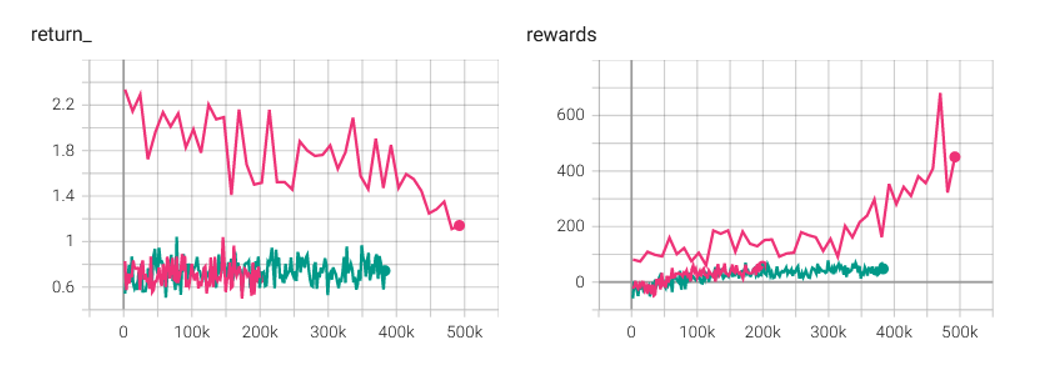
\includegraphics[width=0.79\textwidth]{graphics/fig-three-bad.png}
    \caption{Rewards and returns (PPO) when using state space with three values. The declining pink line in \texttt{return\_}, corresponds to the upper pink line in \texttt{reward}, appeared when Sortino is involved in reward calculation. The $x$-axis indicates the number of timesteps of learning.}
    \label{fig-three-bad}
\end{figure}

\subsection{Reward Function}
	\label{rewardfn}
The reward function for both continuous and discrete action spaces is described using Algorithm \ref{algoreward}.

\begin{algorithm}[h]
\SetAlgoLined
\KwIn{action type}
\KwOut{reward}

\eIf{action = \texttt{BUY}}{
reward $\leftarrow$ 0;
}{
\eIf{action = \texttt{SELL}}{
$reward\_profit \leftarrow sold\_amount \times (sell\_price - average\_held\_price) / average\_held\_price$ \;
$reward\_mdd \leftarrow (latest\_mdd - current\_mdd) \times 0.5$ \;
$reward \leftarrow reward\_profit + reward\_mdd$ \;
}{
$reward\_profit \leftarrow hold\_amount \times (0.0001 * (net\_worth - initial\_balance) / initial\_balance) - 0.0001$ \;
}
}

\KwRet{reward}
\caption{Reward Calculation Algorithm}
\label{algoreward}
\end{algorithm}

There is no reward for buying. Multiplied by the holding amount, holding costs 0.0001 parts of profit or loss added with a flat -0.0001 points of reward to avoid lazy trading: a condition where the agent becomes hesitant to trade to avoid loss, plus a small amount of reduction when the unrealized profit is in the negative zone. When selling, two kinds of rewards are added together. The first component is profit reward, which is the difference between the selling price and the average holding price relative to the average holding price. The last component is how much MDD increases after the selling action times 0.5 to give it less priority than profit reward. The two components are multiplied by the selling amount.

Like determining state space and also mentioned in Fig. \ref{fig-three-bad}, Sortino was originally included in the reward calculation, but was removed due to poor performance.

\subsection{Training And Testing Process}
Each agent is trained 10 times through the training dataset $\mathcal{D}_{train}$. Since each training would likely to return distinct results, one which visually produces the highest return would be handpicked to be the representative of the algorithm. From each agent, a final model would be taken to be tested with all test datasets (\texttt{HBr}, \texttt{HBu}, \texttt{MCr}, \texttt{MBu}).
